% Created by tikzDevice version 0.12.3.2 on 2022-02-18 15:41:58
% !TEX encoding = UTF-8 Unicode
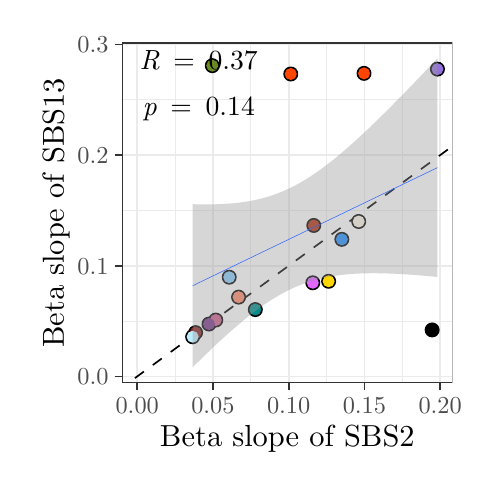
\begin{tikzpicture}[x=1pt,y=1pt]
\definecolor{fillColor}{RGB}{255,255,255}
\path[use as bounding box,fill=fillColor,fill opacity=0.00] (0,0) rectangle (158.99,158.99);
\begin{scope}
\path[clip] (  0.00,  0.00) rectangle (158.99,158.99);
\definecolor{drawColor}{RGB}{255,255,255}
\definecolor{fillColor}{RGB}{255,255,255}

\path[draw=drawColor,line width= 0.6pt,line join=round,line cap=round,fill=fillColor] (  0.00,  0.00) rectangle (158.99,158.99);
\end{scope}
\begin{scope}
\path[clip] ( 34.16, 30.69) rectangle (153.49,153.49);
\definecolor{fillColor}{RGB}{255,255,255}

\path[fill=fillColor] ( 34.16, 30.69) rectangle (153.49,153.49);
\definecolor{drawColor}{gray}{0.92}

\path[draw=drawColor,line width= 0.3pt,line join=round] ( 34.16, 52.95) --
	(153.49, 52.95);

\path[draw=drawColor,line width= 0.3pt,line join=round] ( 34.16, 92.93) --
	(153.49, 92.93);

\path[draw=drawColor,line width= 0.3pt,line join=round] ( 34.16,132.91) --
	(153.49,132.91);

\path[draw=drawColor,line width= 0.3pt,line join=round] ( 53.26, 30.69) --
	( 53.26,153.49);

\path[draw=drawColor,line width= 0.3pt,line join=round] ( 80.63, 30.69) --
	( 80.63,153.49);

\path[draw=drawColor,line width= 0.3pt,line join=round] (108.00, 30.69) --
	(108.00,153.49);

\path[draw=drawColor,line width= 0.3pt,line join=round] (135.36, 30.69) --
	(135.36,153.49);

\path[draw=drawColor,line width= 0.6pt,line join=round] ( 34.16, 32.96) --
	(153.49, 32.96);

\path[draw=drawColor,line width= 0.6pt,line join=round] ( 34.16, 72.94) --
	(153.49, 72.94);

\path[draw=drawColor,line width= 0.6pt,line join=round] ( 34.16,112.92) --
	(153.49,112.92);

\path[draw=drawColor,line width= 0.6pt,line join=round] ( 34.16,152.90) --
	(153.49,152.90);

\path[draw=drawColor,line width= 0.6pt,line join=round] ( 39.58, 30.69) --
	( 39.58,153.49);

\path[draw=drawColor,line width= 0.6pt,line join=round] ( 66.95, 30.69) --
	( 66.95,153.49);

\path[draw=drawColor,line width= 0.6pt,line join=round] ( 94.31, 30.69) --
	( 94.31,153.49);

\path[draw=drawColor,line width= 0.6pt,line join=round] (121.68, 30.69) --
	(121.68,153.49);

\path[draw=drawColor,line width= 0.6pt,line join=round] (149.05, 30.69) --
	(149.05,153.49);
\definecolor{drawColor}{RGB}{0,0,0}

\path[draw=drawColor,line width= 0.6pt,dash pattern=on 4pt off 4pt ,line join=round] (  0.00,  4.05) -- (158.99,120.19);
\definecolor{fillColor}{RGB}{0,0,0}

\path[draw=drawColor,line width= 0.4pt,line join=round,line cap=round,fill=fillColor] (108.75, 67.35) circle (  2.50);

\path[draw=drawColor,line width= 0.4pt,line join=round,line cap=round,fill=fillColor] ( 67.98, 53.34) circle (  2.50);

\path[draw=drawColor,line width= 0.4pt,line join=round,line cap=round,fill=fillColor] (113.52, 82.50) circle (  2.50);

\path[draw=drawColor,line width= 0.4pt,line join=round,line cap=round,fill=fillColor] ( 60.68, 48.80) circle (  2.50);

\path[draw=drawColor,line width= 0.4pt,line join=round,line cap=round,fill=fillColor] (103.38, 87.52) circle (  2.50);

\path[draw=drawColor,line width= 0.4pt,line join=round,line cap=round,fill=fillColor] (121.54,142.48) circle (  2.50);

\path[draw=drawColor,line width= 0.4pt,line join=round,line cap=round,fill=fillColor] ( 95.07,142.25) circle (  2.50);

\path[draw=drawColor,line width= 0.4pt,line join=round,line cap=round,fill=fillColor] (119.61, 88.95) circle (  2.50);

\path[draw=drawColor,line width= 0.4pt,line join=round,line cap=round,fill=fillColor] ( 66.71,145.26) circle (  2.50);

\path[draw=drawColor,line width= 0.4pt,line join=round,line cap=round,fill=fillColor] ( 82.26, 57.13) circle (  2.50);

\path[draw=drawColor,line width= 0.4pt,line join=round,line cap=round,fill=fillColor] ( 65.51, 51.89) circle (  2.50);

\path[draw=drawColor,line width= 0.4pt,line join=round,line cap=round,fill=fillColor] (103.03, 66.80) circle (  2.50);

\path[draw=drawColor,line width= 0.4pt,line join=round,line cap=round,fill=fillColor] ( 72.83, 68.82) circle (  2.50);

\path[draw=drawColor,line width= 0.4pt,line join=round,line cap=round,fill=fillColor] (146.15, 49.77) circle (  2.50);

\path[draw=drawColor,line width= 0.4pt,line join=round,line cap=round,fill=fillColor] ( 59.61, 47.29) circle (  2.50);

\path[draw=drawColor,line width= 0.4pt,line join=round,line cap=round,fill=fillColor] (148.07,144.01) circle (  2.50);

\path[draw=drawColor,line width= 0.4pt,line join=round,line cap=round,fill=fillColor] ( 76.21, 61.62) circle (  2.50);
\definecolor{drawColor}{RGB}{255,215,0}
\definecolor{fillColor}{RGB}{255,215,0}

\path[draw=drawColor,line width= 0.4pt,line join=round,line cap=round,fill=fillColor] (108.75, 67.35) circle (  1.96);
\definecolor{drawColor}{RGB}{205,96,144}
\definecolor{fillColor}{RGB}{205,96,144}

\path[draw=drawColor,line width= 0.4pt,line join=round,line cap=round,fill=fillColor] ( 67.98, 53.34) circle (  1.96);
\definecolor{drawColor}{RGB}{30,144,255}
\definecolor{fillColor}{RGB}{30,144,255}

\path[draw=drawColor,line width= 0.4pt,line join=round,line cap=round,fill=fillColor] (113.52, 82.50) circle (  1.96);
\definecolor{drawColor}{RGB}{139,35,35}
\definecolor{fillColor}{RGB}{139,35,35}

\path[draw=drawColor,line width= 0.4pt,line join=round,line cap=round,fill=fillColor] ( 60.68, 48.80) circle (  1.96);
\definecolor{drawColor}{RGB}{179,47,11}
\definecolor{fillColor}{RGB}{179,47,11}

\path[draw=drawColor,line width= 0.4pt,line join=round,line cap=round,fill=fillColor] (103.38, 87.52) circle (  1.96);
\definecolor{drawColor}{RGB}{255,69,0}
\definecolor{fillColor}{RGB}{255,69,0}

\path[draw=drawColor,line width= 0.4pt,line join=round,line cap=round,fill=fillColor] (121.54,142.48) circle (  1.96);

\path[draw=drawColor,line width= 0.4pt,line join=round,line cap=round,fill=fillColor] ( 95.07,142.25) circle (  1.96);
\definecolor{drawColor}{RGB}{253,245,230}
\definecolor{fillColor}{RGB}{253,245,230}

\path[draw=drawColor,line width= 0.4pt,line join=round,line cap=round,fill=fillColor] (119.61, 88.95) circle (  1.96);
\definecolor{drawColor}{RGB}{105,139,34}
\definecolor{fillColor}{RGB}{105,139,34}

\path[draw=drawColor,line width= 0.4pt,line join=round,line cap=round,fill=fillColor] ( 66.71,145.26) circle (  1.96);
\definecolor{drawColor}{RGB}{0,139,139}
\definecolor{fillColor}{RGB}{0,139,139}

\path[draw=drawColor,line width= 0.4pt,line join=round,line cap=round,fill=fillColor] ( 82.26, 57.13) circle (  1.96);
\definecolor{drawColor}{RGB}{122,55,139}
\definecolor{fillColor}{RGB}{122,55,139}

\path[draw=drawColor,line width= 0.4pt,line join=round,line cap=round,fill=fillColor] ( 65.51, 51.89) circle (  1.96);
\definecolor{drawColor}{RGB}{224,102,255}
\definecolor{fillColor}{RGB}{224,102,255}

\path[draw=drawColor,line width= 0.4pt,line join=round,line cap=round,fill=fillColor] (103.03, 66.80) circle (  1.96);
\definecolor{drawColor}{RGB}{135,206,250}
\definecolor{fillColor}{RGB}{135,206,250}

\path[draw=drawColor,line width= 0.4pt,line join=round,line cap=round,fill=fillColor] ( 72.83, 68.82) circle (  1.96);
\definecolor{drawColor}{RGB}{0,0,0}
\definecolor{fillColor}{RGB}{0,0,0}

\path[draw=drawColor,line width= 0.4pt,line join=round,line cap=round,fill=fillColor] (146.15, 49.77) circle (  1.96);
\definecolor{drawColor}{RGB}{191,239,255}
\definecolor{fillColor}{RGB}{191,239,255}

\path[draw=drawColor,line width= 0.4pt,line join=round,line cap=round,fill=fillColor] ( 59.61, 47.29) circle (  1.96);
\definecolor{drawColor}{RGB}{147,112,219}
\definecolor{fillColor}{RGB}{147,112,219}

\path[draw=drawColor,line width= 0.4pt,line join=round,line cap=round,fill=fillColor] (148.07,144.01) circle (  1.96);
\definecolor{drawColor}{RGB}{255,140,105}
\definecolor{fillColor}{RGB}{255,140,105}

\path[draw=drawColor,line width= 0.4pt,line join=round,line cap=round,fill=fillColor] ( 76.21, 61.62) circle (  1.96);
\definecolor{fillColor}{RGB}{153,153,153}

\path[fill=fillColor,fill opacity=0.40] ( 59.61, 95.21) --
	( 60.73, 95.17) --
	( 61.85, 95.15) --
	( 62.97, 95.13) --
	( 64.09, 95.13) --
	( 65.21, 95.13) --
	( 66.33, 95.14) --
	( 67.45, 95.16) --
	( 68.57, 95.19) --
	( 69.69, 95.23) --
	( 70.81, 95.29) --
	( 71.93, 95.35) --
	( 73.05, 95.44) --
	( 74.17, 95.53) --
	( 75.29, 95.64) --
	( 76.40, 95.77) --
	( 77.52, 95.92) --
	( 78.64, 96.08) --
	( 79.76, 96.26) --
	( 80.88, 96.46) --
	( 82.00, 96.69) --
	( 83.12, 96.93) --
	( 84.24, 97.20) --
	( 85.36, 97.50) --
	( 86.48, 97.81) --
	( 87.60, 98.16) --
	( 88.72, 98.53) --
	( 89.84, 98.93) --
	( 90.96, 99.36) --
	( 92.08, 99.81) --
	( 93.20,100.30) --
	( 94.32,100.81) --
	( 95.44,101.35) --
	( 96.56,101.92) --
	( 97.68,102.53) --
	( 98.80,103.16) --
	( 99.92,103.82) --
	(101.04,104.51) --
	(102.16,105.22) --
	(103.28,105.96) --
	(104.40,106.73) --
	(105.52,107.52) --
	(106.64,108.34) --
	(107.76,109.18) --
	(108.88,110.04) --
	(110.00,110.92) --
	(111.12,111.82) --
	(112.24,112.74) --
	(113.36,113.68) --
	(114.48,114.64) --
	(115.60,115.61) --
	(116.72,116.60) --
	(117.84,117.60) --
	(118.96,118.62) --
	(120.08,119.64) --
	(121.20,120.68) --
	(122.32,121.73) --
	(123.43,122.80) --
	(124.55,123.87) --
	(125.67,124.95) --
	(126.79,126.04) --
	(127.91,127.14) --
	(129.03,128.24) --
	(130.15,129.36) --
	(131.27,130.48) --
	(132.39,131.61) --
	(133.51,132.74) --
	(134.63,133.88) --
	(135.75,135.02) --
	(136.87,136.17) --
	(137.99,137.33) --
	(139.11,138.49) --
	(140.23,139.65) --
	(141.35,140.82) --
	(142.47,142.00) --
	(143.59,143.17) --
	(144.71,144.35) --
	(145.83,145.54) --
	(146.95,146.72) --
	(148.07,147.91) --
	(148.07, 68.90) --
	(146.95, 69.01) --
	(145.83, 69.12) --
	(144.71, 69.22) --
	(143.59, 69.32) --
	(142.47, 69.42) --
	(141.35, 69.51) --
	(140.23, 69.60) --
	(139.11, 69.68) --
	(137.99, 69.76) --
	(136.87, 69.84) --
	(135.75, 69.91) --
	(134.63, 69.97) --
	(133.51, 70.03) --
	(132.39, 70.08) --
	(131.27, 70.13) --
	(130.15, 70.17) --
	(129.03, 70.21) --
	(127.91, 70.23) --
	(126.79, 70.25) --
	(125.67, 70.26) --
	(124.55, 70.26) --
	(123.43, 70.25) --
	(122.32, 70.23) --
	(121.20, 70.20) --
	(120.08, 70.16) --
	(118.96, 70.11) --
	(117.84, 70.05) --
	(116.72, 69.97) --
	(115.60, 69.88) --
	(114.48, 69.77) --
	(113.36, 69.64) --
	(112.24, 69.50) --
	(111.12, 69.34) --
	(110.00, 69.16) --
	(108.88, 68.97) --
	(107.76, 68.75) --
	(106.64, 68.51) --
	(105.52, 68.24) --
	(104.40, 67.95) --
	(103.28, 67.64) --
	(102.16, 67.30) --
	(101.04, 66.94) --
	( 99.92, 66.55) --
	( 98.80, 66.12) --
	( 97.68, 65.68) --
	( 96.56, 65.20) --
	( 95.44, 64.69) --
	( 94.32, 64.15) --
	( 93.20, 63.59) --
	( 92.08, 62.99) --
	( 90.96, 62.37) --
	( 89.84, 61.71) --
	( 88.72, 61.03) --
	( 87.60, 60.32) --
	( 86.48, 59.59) --
	( 85.36, 58.82) --
	( 84.24, 58.04) --
	( 83.12, 57.22) --
	( 82.00, 56.39) --
	( 80.88, 55.53) --
	( 79.76, 54.66) --
	( 78.64, 53.76) --
	( 77.52, 52.84) --
	( 76.40, 51.91) --
	( 75.29, 50.95) --
	( 74.17, 49.98) --
	( 73.05, 49.00) --
	( 71.93, 48.00) --
	( 70.81, 46.99) --
	( 69.69, 45.96) --
	( 68.57, 44.93) --
	( 67.45, 43.88) --
	( 66.33, 42.82) --
	( 65.21, 41.75) --
	( 64.09, 40.67) --
	( 62.97, 39.58) --
	( 61.85, 38.48) --
	( 60.73, 37.38) --
	( 59.61, 36.27) --
	cycle;

\path[] ( 59.61, 95.21) --
	( 60.73, 95.17) --
	( 61.85, 95.15) --
	( 62.97, 95.13) --
	( 64.09, 95.13) --
	( 65.21, 95.13) --
	( 66.33, 95.14) --
	( 67.45, 95.16) --
	( 68.57, 95.19) --
	( 69.69, 95.23) --
	( 70.81, 95.29) --
	( 71.93, 95.35) --
	( 73.05, 95.44) --
	( 74.17, 95.53) --
	( 75.29, 95.64) --
	( 76.40, 95.77) --
	( 77.52, 95.92) --
	( 78.64, 96.08) --
	( 79.76, 96.26) --
	( 80.88, 96.46) --
	( 82.00, 96.69) --
	( 83.12, 96.93) --
	( 84.24, 97.20) --
	( 85.36, 97.50) --
	( 86.48, 97.81) --
	( 87.60, 98.16) --
	( 88.72, 98.53) --
	( 89.84, 98.93) --
	( 90.96, 99.36) --
	( 92.08, 99.81) --
	( 93.20,100.30) --
	( 94.32,100.81) --
	( 95.44,101.35) --
	( 96.56,101.92) --
	( 97.68,102.53) --
	( 98.80,103.16) --
	( 99.92,103.82) --
	(101.04,104.51) --
	(102.16,105.22) --
	(103.28,105.96) --
	(104.40,106.73) --
	(105.52,107.52) --
	(106.64,108.34) --
	(107.76,109.18) --
	(108.88,110.04) --
	(110.00,110.92) --
	(111.12,111.82) --
	(112.24,112.74) --
	(113.36,113.68) --
	(114.48,114.64) --
	(115.60,115.61) --
	(116.72,116.60) --
	(117.84,117.60) --
	(118.96,118.62) --
	(120.08,119.64) --
	(121.20,120.68) --
	(122.32,121.73) --
	(123.43,122.80) --
	(124.55,123.87) --
	(125.67,124.95) --
	(126.79,126.04) --
	(127.91,127.14) --
	(129.03,128.24) --
	(130.15,129.36) --
	(131.27,130.48) --
	(132.39,131.61) --
	(133.51,132.74) --
	(134.63,133.88) --
	(135.75,135.02) --
	(136.87,136.17) --
	(137.99,137.33) --
	(139.11,138.49) --
	(140.23,139.65) --
	(141.35,140.82) --
	(142.47,142.00) --
	(143.59,143.17) --
	(144.71,144.35) --
	(145.83,145.54) --
	(146.95,146.72) --
	(148.07,147.91);

\path[] (148.07, 68.90) --
	(146.95, 69.01) --
	(145.83, 69.12) --
	(144.71, 69.22) --
	(143.59, 69.32) --
	(142.47, 69.42) --
	(141.35, 69.51) --
	(140.23, 69.60) --
	(139.11, 69.68) --
	(137.99, 69.76) --
	(136.87, 69.84) --
	(135.75, 69.91) --
	(134.63, 69.97) --
	(133.51, 70.03) --
	(132.39, 70.08) --
	(131.27, 70.13) --
	(130.15, 70.17) --
	(129.03, 70.21) --
	(127.91, 70.23) --
	(126.79, 70.25) --
	(125.67, 70.26) --
	(124.55, 70.26) --
	(123.43, 70.25) --
	(122.32, 70.23) --
	(121.20, 70.20) --
	(120.08, 70.16) --
	(118.96, 70.11) --
	(117.84, 70.05) --
	(116.72, 69.97) --
	(115.60, 69.88) --
	(114.48, 69.77) --
	(113.36, 69.64) --
	(112.24, 69.50) --
	(111.12, 69.34) --
	(110.00, 69.16) --
	(108.88, 68.97) --
	(107.76, 68.75) --
	(106.64, 68.51) --
	(105.52, 68.24) --
	(104.40, 67.95) --
	(103.28, 67.64) --
	(102.16, 67.30) --
	(101.04, 66.94) --
	( 99.92, 66.55) --
	( 98.80, 66.12) --
	( 97.68, 65.68) --
	( 96.56, 65.20) --
	( 95.44, 64.69) --
	( 94.32, 64.15) --
	( 93.20, 63.59) --
	( 92.08, 62.99) --
	( 90.96, 62.37) --
	( 89.84, 61.71) --
	( 88.72, 61.03) --
	( 87.60, 60.32) --
	( 86.48, 59.59) --
	( 85.36, 58.82) --
	( 84.24, 58.04) --
	( 83.12, 57.22) --
	( 82.00, 56.39) --
	( 80.88, 55.53) --
	( 79.76, 54.66) --
	( 78.64, 53.76) --
	( 77.52, 52.84) --
	( 76.40, 51.91) --
	( 75.29, 50.95) --
	( 74.17, 49.98) --
	( 73.05, 49.00) --
	( 71.93, 48.00) --
	( 70.81, 46.99) --
	( 69.69, 45.96) --
	( 68.57, 44.93) --
	( 67.45, 43.88) --
	( 66.33, 42.82) --
	( 65.21, 41.75) --
	( 64.09, 40.67) --
	( 62.97, 39.58) --
	( 61.85, 38.48) --
	( 60.73, 37.38) --
	( 59.61, 36.27);
\definecolor{drawColor}{RGB}{51,102,255}

\path[draw=drawColor,line width= 0.2pt,line join=round] ( 59.61, 65.74) --
	( 60.73, 66.28) --
	( 61.85, 66.82) --
	( 62.97, 67.36) --
	( 64.09, 67.90) --
	( 65.21, 68.44) --
	( 66.33, 68.98) --
	( 67.45, 69.52) --
	( 68.57, 70.06) --
	( 69.69, 70.60) --
	( 70.81, 71.14) --
	( 71.93, 71.68) --
	( 73.05, 72.22) --
	( 74.17, 72.76) --
	( 75.29, 73.30) --
	( 76.40, 73.84) --
	( 77.52, 74.38) --
	( 78.64, 74.92) --
	( 79.76, 75.46) --
	( 80.88, 76.00) --
	( 82.00, 76.54) --
	( 83.12, 77.08) --
	( 84.24, 77.62) --
	( 85.36, 78.16) --
	( 86.48, 78.70) --
	( 87.60, 79.24) --
	( 88.72, 79.78) --
	( 89.84, 80.32) --
	( 90.96, 80.86) --
	( 92.08, 81.40) --
	( 93.20, 81.94) --
	( 94.32, 82.48) --
	( 95.44, 83.02) --
	( 96.56, 83.56) --
	( 97.68, 84.10) --
	( 98.80, 84.64) --
	( 99.92, 85.18) --
	(101.04, 85.72) --
	(102.16, 86.26) --
	(103.28, 86.80) --
	(104.40, 87.34) --
	(105.52, 87.88) --
	(106.64, 88.42) --
	(107.76, 88.96) --
	(108.88, 89.50) --
	(110.00, 90.04) --
	(111.12, 90.58) --
	(112.24, 91.12) --
	(113.36, 91.66) --
	(114.48, 92.20) --
	(115.60, 92.74) --
	(116.72, 93.28) --
	(117.84, 93.82) --
	(118.96, 94.36) --
	(120.08, 94.90) --
	(121.20, 95.44) --
	(122.32, 95.98) --
	(123.43, 96.52) --
	(124.55, 97.06) --
	(125.67, 97.60) --
	(126.79, 98.14) --
	(127.91, 98.68) --
	(129.03, 99.22) --
	(130.15, 99.76) --
	(131.27,100.30) --
	(132.39,100.84) --
	(133.51,101.39) --
	(134.63,101.93) --
	(135.75,102.47) --
	(136.87,103.01) --
	(137.99,103.55) --
	(139.11,104.09) --
	(140.23,104.63) --
	(141.35,105.17) --
	(142.47,105.71) --
	(143.59,106.25) --
	(144.71,106.79) --
	(145.83,107.33) --
	(146.95,107.87) --
	(148.07,108.41);
\definecolor{drawColor}{RGB}{0,0,0}

\node[text=drawColor,anchor=base west,inner sep=0pt, outer sep=0pt, scale=  1.00] at ( 40.43,143.99) {\itshape R};

\node[text=drawColor,anchor=base west,inner sep=0pt, outer sep=0pt, scale=  1.00] at ( 47.70,143.99) { };

\node[text=drawColor,anchor=base west,inner sep=0pt, outer sep=0pt, scale=  1.00] at ( 52.67,143.99) {=};

\node[text=drawColor,anchor=base west,inner sep=0pt, outer sep=0pt, scale=  1.00] at ( 60.42,143.99) { };

\node[text=drawColor,anchor=base west,inner sep=0pt, outer sep=0pt, scale=  1.00] at ( 65.39,143.99) {0.37};

\node[text=drawColor,anchor=base west,inner sep=0pt, outer sep=0pt, scale=  1.00] at ( 41.52,127.16) {\itshape p};

\node[text=drawColor,anchor=base west,inner sep=0pt, outer sep=0pt, scale=  1.00] at ( 46.61,127.16) { };

\node[text=drawColor,anchor=base west,inner sep=0pt, outer sep=0pt, scale=  1.00] at ( 51.59,127.16) {=};

\node[text=drawColor,anchor=base west,inner sep=0pt, outer sep=0pt, scale=  1.00] at ( 59.33,127.16) { };

\node[text=drawColor,anchor=base west,inner sep=0pt, outer sep=0pt, scale=  1.00] at ( 64.31,127.16) {0.14};
\definecolor{drawColor}{gray}{0.20}

\path[draw=drawColor,line width= 0.6pt,line join=round,line cap=round] ( 34.16, 30.69) rectangle (153.49,153.49);
\end{scope}
\begin{scope}
\path[clip] (  0.00,  0.00) rectangle (158.99,158.99);
\definecolor{drawColor}{gray}{0.30}

\node[text=drawColor,anchor=base east,inner sep=0pt, outer sep=0pt, scale=  0.88] at ( 29.21, 29.93) {0.0};

\node[text=drawColor,anchor=base east,inner sep=0pt, outer sep=0pt, scale=  0.88] at ( 29.21, 69.91) {0.1};

\node[text=drawColor,anchor=base east,inner sep=0pt, outer sep=0pt, scale=  0.88] at ( 29.21,109.89) {0.2};

\node[text=drawColor,anchor=base east,inner sep=0pt, outer sep=0pt, scale=  0.88] at ( 29.21,149.87) {0.3};
\end{scope}
\begin{scope}
\path[clip] (  0.00,  0.00) rectangle (158.99,158.99);
\definecolor{drawColor}{gray}{0.20}

\path[draw=drawColor,line width= 0.6pt,line join=round] ( 31.41, 32.96) --
	( 34.16, 32.96);

\path[draw=drawColor,line width= 0.6pt,line join=round] ( 31.41, 72.94) --
	( 34.16, 72.94);

\path[draw=drawColor,line width= 0.6pt,line join=round] ( 31.41,112.92) --
	( 34.16,112.92);

\path[draw=drawColor,line width= 0.6pt,line join=round] ( 31.41,152.90) --
	( 34.16,152.90);
\end{scope}
\begin{scope}
\path[clip] (  0.00,  0.00) rectangle (158.99,158.99);
\definecolor{drawColor}{gray}{0.20}

\path[draw=drawColor,line width= 0.6pt,line join=round] ( 39.58, 27.94) --
	( 39.58, 30.69);

\path[draw=drawColor,line width= 0.6pt,line join=round] ( 66.95, 27.94) --
	( 66.95, 30.69);

\path[draw=drawColor,line width= 0.6pt,line join=round] ( 94.31, 27.94) --
	( 94.31, 30.69);

\path[draw=drawColor,line width= 0.6pt,line join=round] (121.68, 27.94) --
	(121.68, 30.69);

\path[draw=drawColor,line width= 0.6pt,line join=round] (149.05, 27.94) --
	(149.05, 30.69);
\end{scope}
\begin{scope}
\path[clip] (  0.00,  0.00) rectangle (158.99,158.99);
\definecolor{drawColor}{gray}{0.30}

\node[text=drawColor,anchor=base,inner sep=0pt, outer sep=0pt, scale=  0.88] at ( 39.58, 19.68) {0.00};

\node[text=drawColor,anchor=base,inner sep=0pt, outer sep=0pt, scale=  0.88] at ( 66.95, 19.68) {0.05};

\node[text=drawColor,anchor=base,inner sep=0pt, outer sep=0pt, scale=  0.88] at ( 94.31, 19.68) {0.10};

\node[text=drawColor,anchor=base,inner sep=0pt, outer sep=0pt, scale=  0.88] at (121.68, 19.68) {0.15};

\node[text=drawColor,anchor=base,inner sep=0pt, outer sep=0pt, scale=  0.88] at (149.05, 19.68) {0.20};
\end{scope}
\begin{scope}
\path[clip] (  0.00,  0.00) rectangle (158.99,158.99);
\definecolor{drawColor}{RGB}{0,0,0}

\node[text=drawColor,anchor=base,inner sep=0pt, outer sep=0pt, scale=  1.10] at ( 93.83,  7.64) {Beta slope of SBS2};
\end{scope}
\begin{scope}
\path[clip] (  0.00,  0.00) rectangle (158.99,158.99);
\definecolor{drawColor}{RGB}{0,0,0}

\node[text=drawColor,rotate= 90.00,anchor=base,inner sep=0pt, outer sep=0pt, scale=  1.10] at ( 13.08, 92.09) {Beta slope of SBS13};
\end{scope}
\end{tikzpicture}
